%!TEX root = ../NCVC7.tex
\mysection{3D-CADデータの準備}

\subsection{IGESデータについて}
\label{sec:AboutIGES}
 現状のKodatunoライブラリで処理できるIGESデータは,NURBSの曲線と曲面のみです.
お使いのCADデータからIGESデータを出力する際は,NURBSオプションを選択してください.
Kodatunoライブラリ開発元からの情報によると,SolidWorks, SolidEdge, CATIAから出力されたIGESデータは問題なく読めるようです.
InventorからのIGESデータは読めないとのことでした.

 筆者は Rhinoceros で動作確認しています\footnote{特段推奨しているわけではありません.}.
Rhinoceros から出力されるIGESデータも問題なく読めましたが,
一部NCVCが落ちるデータも確認しました\footnote{try-catchブロックでも捉えられない例外エラーでNCVCが落ちてしまいます.調査継続中.}.
保存時のIGESタイプを変更すると読める場合もあったので,適宜対応してください.

\subsection{原点について}
 2D-CADデータのときは『ORIGINレイヤに円を作図』というNCVCの独自ルールがありましたが,
3D-CADデータの場合は作図原点がそのまま加工原点(工具の初期位置)になります.
ただし,Z値については後述する設定でワーク上面をゼロにすることが可能です.

\subsection{スキャニングパス生成用のガイドカーブ}
 スキャニングパスの生成では,基準となるガイドカーブ(NURBS曲線)が必要です.
3Dモデルを囲うように作図してください.
ガイドカーブが円だとスキャニングパスがうまく生成できないことを確認しています.

\begin{figure}[H]
\centering
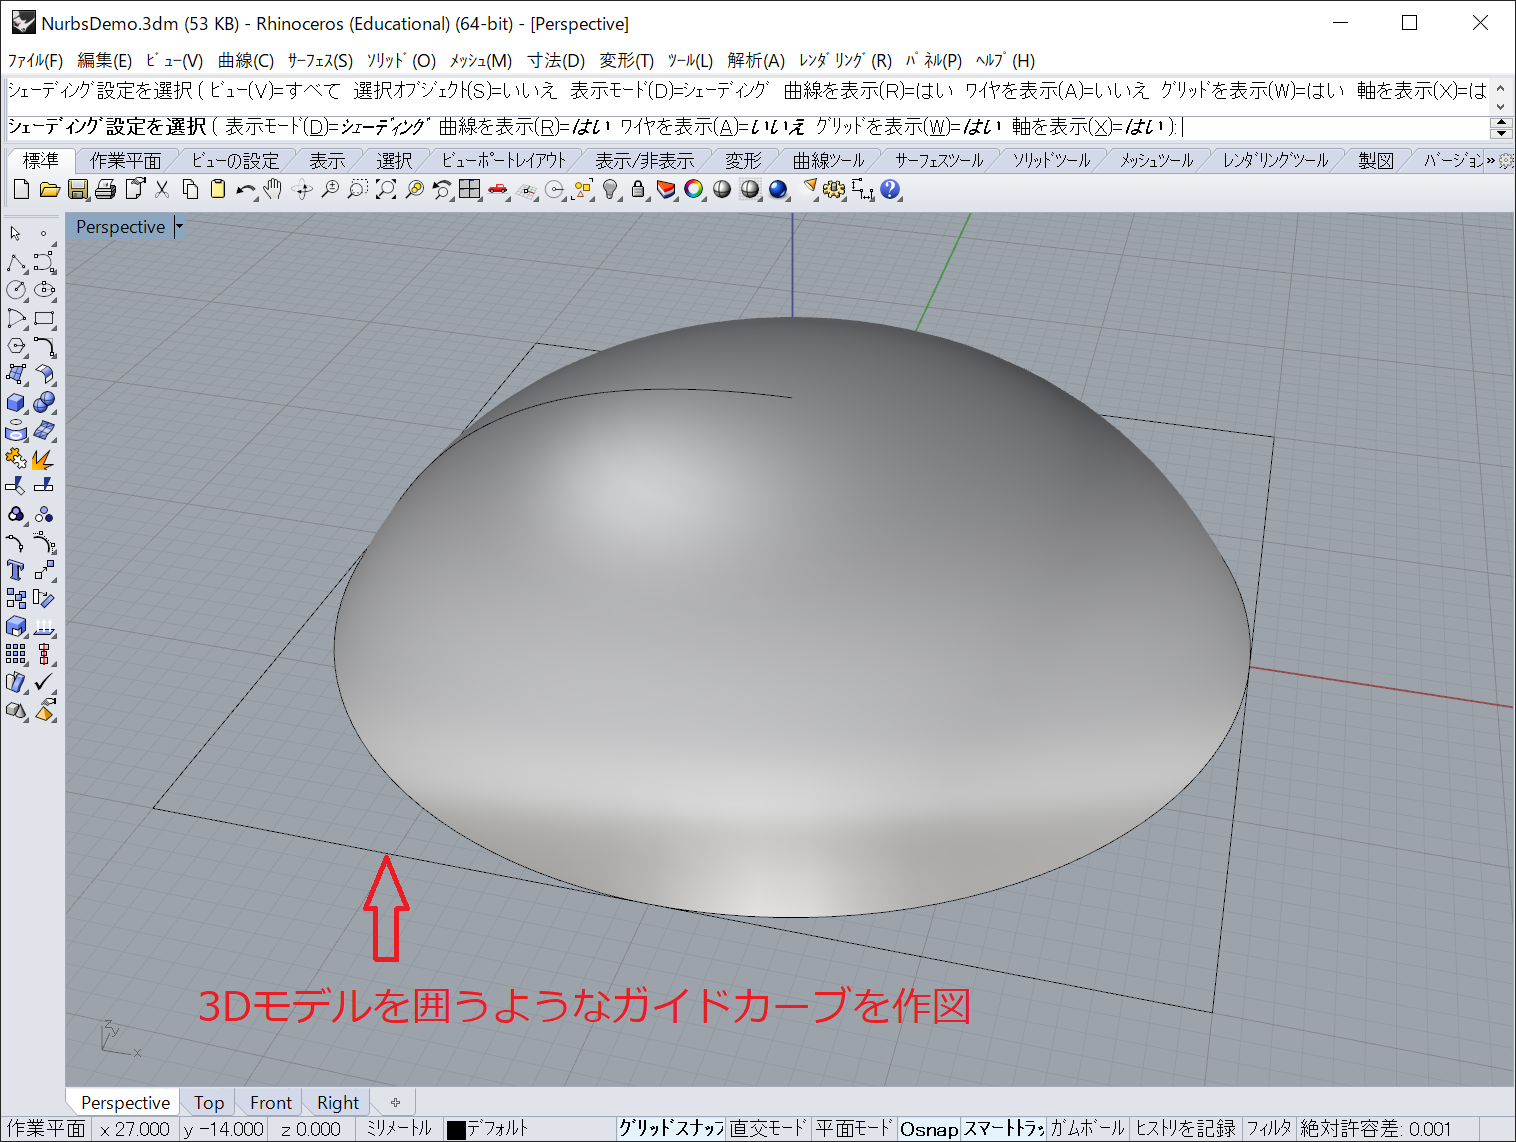
\includegraphics[scale=0.5]{No1/fig/fig11.png}
\caption{サンプル図形}
\label{fig:sample.iges}
\end{figure}

\subsection{NCVCの設定ファイルについて}
 IGESデータと同じ場所に,NCVCの設定ファイル(~.ncvc)が自動的に作られます.
インストーラ付属のサンプルデータを使用する場合は,ドキュメントフォルダ等の書き込み権限がある場所にコピーしてから使用してください.

\subsection{Kodatunoライブラリからのメッセージ}
\label{sec:KodatunoMsg}
 計算処理の途中でKodatunoライブラリからメッセージが表示されることがあります.
データが欠落していたり,おかしなパスが生成される場合があるので,とくにご注意ください.
3Dモデルを変更したり,生成後のデータを手作業で修正する必要があるかもしれません.

\begin{table}[H]
\centering
\caption{Kodatunoライブラリのメッセージ一覧}
\label{tab:kodatuno_msg}
\begin{tabular}{l|l}
\hline
\texttt{NURBS\_FUNC CAUTION: Singler point was ditected.} & 特異点検出により処理を継続できない場合 \\ \hline
\texttt{NURBS KOD\_ERROR: Intersection points exceeded the} & 交点の数が指定サイズを超えた場合は \\
\texttt{allocated array length. There is a possibility} & そこまでで強制リターン \\
\texttt{that you set large ds.} & \\ \hline
\end{tabular}
\end{table}
